\documentclass[t,noamsthm]{beamer}

\mode<presentation>{
  \usetheme{default}

  \setbeamercolor{normal text}{fg=white,bg=black}
  \setbeamercolor{structure}{fg=orange!80!white}

  \setbeamercolor{alerted text}{use=structure,fg=structure.fg!50!red}

  \setbeamercolor{item projected}{use=item,fg=black,bg=item.fg!75}

  \setbeamercolor*{sidebar}{bg=black!50}

  \setbeamercolor*{palette primary}{use=structure,fg=structure.fg}
  \setbeamercolor*{palette secondary}{use=structure,fg=structure.fg!95!black}
  \setbeamercolor*{palette tertiary}{use=structure,fg=structure.fg!90!black}
  \setbeamercolor*{palette quaternary}{use=structure,fg=structure.fg!85!black}

  \setbeamercolor*{framesubtitle}{fg=white}
  \setbeamercolor*{subtitle}{fg=white}
  \setbeamercolor*{title}{fg=orange}

  \setbeamercolor*{block title}{parent=structure,fg=orange}
  \setbeamercolor*{block title alerted}{parent=alerted text}
  \setbeamercolor*{block title example}{parent=example text}

  \setbeamertemplate{navigation symbols}{}
  \setbeamertemplate{footline}[frame number]

  \setbeamertemplate{background}{
    \begin{tikzpicture}<0->[overlay, remember picture]
      \path (current page.north west) rectangle (current page.south east);
      \node[above right=3pt, opacity=0.5] at (current page.south west) {
        
\includegraphics[width=35mm]{rackspace-logo}
      };
    \end{tikzpicture}
  }

  \pdfcatalog{/PageLayout /SinglePage}
}
\mode<handout>{
  \usepackage{pgfpages}
  \pgfpagesuselayout{4 on 1}[a4paper,landscape,border shrink=3mm]
  %\pgfpagesuselayout{8 on 1}[a4paper]
}

\usepackage[english]{babel}
\usepackage[latin1]{inputenc}
\usepackage[T1]{fontenc}
\usepackage{lmodern,textcomp}

\title{Swift Browser: an AngularJS Swift Client}
\subtitle{https://github.com/zerovm/swift-browser/}
\author{Martin Geisler}
\institute{Rackspace International,\\Zurich Switzerland}
\date{March 30th, 2015}

% If you wish to uncover everything in a step-wise fashion, uncomment
% the following command:
%\beamerdefaultoverlayspecification{<+->}

\usepackage{graphicx}

\usepackage{tikz}
%\usetikzlibrary{positioning}
%\usetikzlibrary{calc}
%\usetikzlibrary{shapes.symbols}

\pgfdeclarelayer{background}
\pgfdeclarelayer{foreground}
\pgfsetlayers{background,main,foreground}

\tikzstyle{every entity}=[thick, draw=red!80!white, fill=red!20!structure.bg]
\tikzstyle{every relationship}=[thick, draw=green!80!white,
  fill=green!20!structure.bg]
\tikzstyle{every attribute}=[thick, draw=structure, fill=structure!20!structure.bg]

%\tikzset{every fit/.append style=text badly centered}
%\tikzstyle{every picture}=[thick]
%\tikzstyle{orange}=[draw=structure, fill=structure!20!structure.bg]
%\tikzstyle{red glow}=[draw=red!80!white, fill=red!20!structure.bg]
%\tikzstyle{light red glow}=[draw=red!80!white, fill=red!15!structure.bg]
%\tikzstyle{box}=[
%  orange, text width=18mm, minimum height=12mm, text centered,
%  outer sep=3pt,
%]

\usepackage{listings}

\lstdefinelanguage{JavaScript}{
  keywords={break, case, catch, continue, debugger, default, delete, do, else, false, finally, for, function, if, in, instanceof, new, null, return, switch, this, throw, true, try, typeof, var, void, while, with},
  morecomment=[l]{//},
  morecomment=[s]{/*}{*/},
  morestring=[b]',
  morestring=[b]",
  ndkeywords={class, export, boolean, throw, implements, import, this},
  sensitive=true
}

\lstset{
  language=JavaScript,
  basicstyle=\footnotesize,
  keywordstyle=\color{structure.fg!50!red},
  stringstyle=\color{structure.fg!70!white},
  columns=fullflexible,
  showstringspaces=false,
  frame=single,
  framerule=0.8pt,
  rulecolor=\color{structure},
  backgroundcolor=\color{structure!10!structure.bg},
  morekeywords={assert,with}
}
\newcommand{\py}[1]{\textcolor{green!70!structure.bg}{#1}}
\newcommand{\code}[1]{#1}


\newcommand{\fixframebreakvspace}{\vspace{-3.75pt}}
\newcommand{\rrrangle}{\texttt{>{}>{}>}}

%\usepackage{nath} \delimgrowth=1
%\mathindent=1em

\AtBeginSection{
  \begin{frame}{Outline}
    \tableofcontents[currentsection]
  \end{frame}
}

\begin{document}

\begin{frame}
  \titlepage
\end{frame}

\begin{frame}{Outline}
  \tableofcontents
\end{frame}

\section{Introduction}

\begin{frame}[c]{OpenStack Components}
  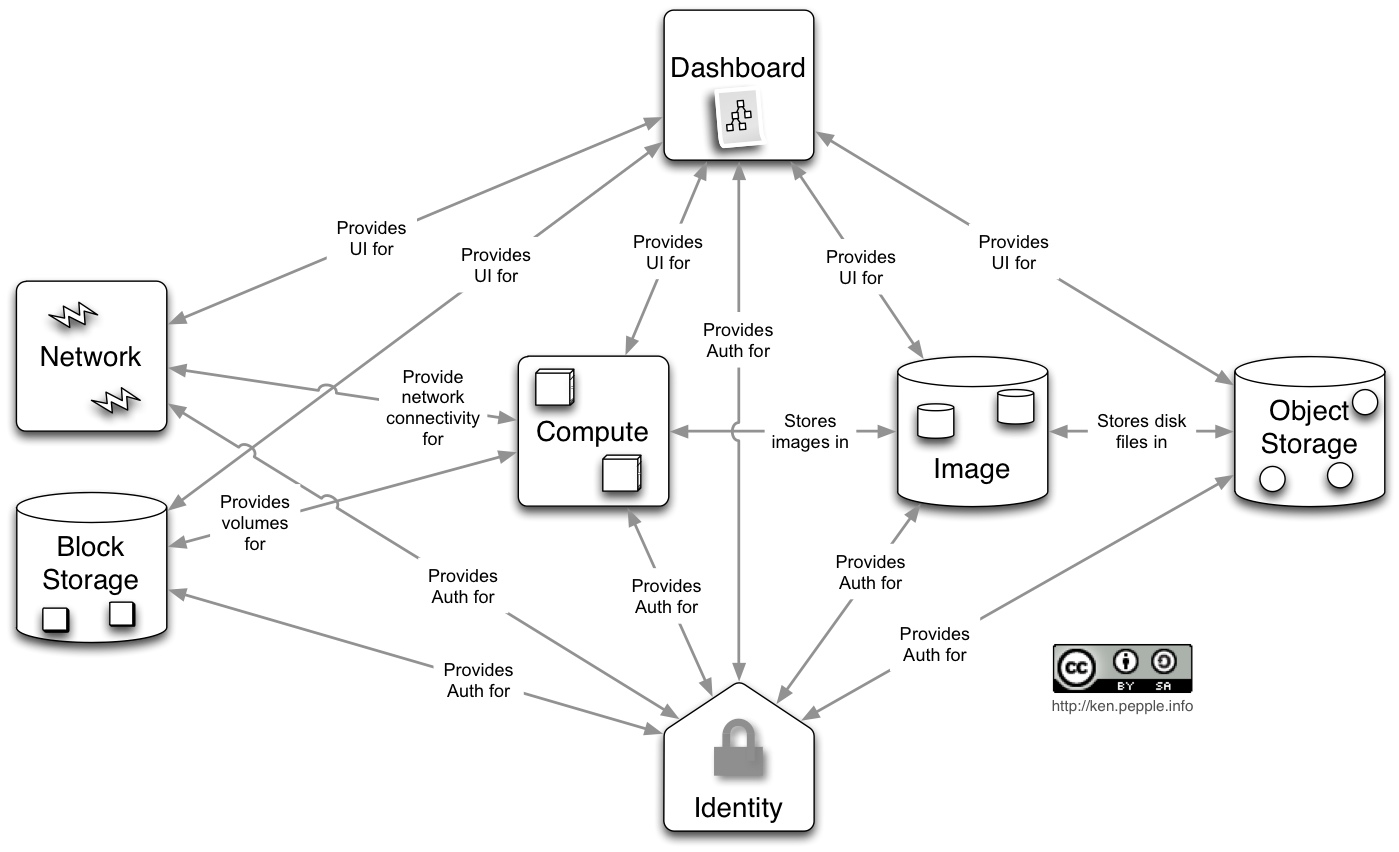
\includegraphics[width=\textwidth]{openstack-components}
\end{frame}

\begin{frame}{OpenStack Swift}
  Scalable object storage:
  \begin{itemize}
  \item stores objects in containers
  \item high-availability thanks to replication
  \item scalable to millions of objects
  \item uses thousands of machines
  \end{itemize}
\end{frame}

\section{Swift API}

\newcommand{\contreq}[1]{\texttt{\makebox[3em][l]{#1} %
    /v1/<account>/<container>}}
\newcommand{\objreq}[1]{\texttt{\makebox[3em][l]{#1} %
    /v1/<account>/<container>/<object>}}

\begin{frame}{Swift Object API}
  Modern REST API for operating on objects:
  \begin{itemize}
  \item \alert<2>{\objreq{GET}}
  \item \objreq{PUT}
  \item \objreq{DELETE}
  \item \objreq{HEAD}
  \item \objreq{POST}
  \end{itemize}

  Full API documentation: \url{http://developer.openstack.org/api-ref-objectstorage-v1.html}.
\end{frame}

\begin{frame}{Swift Container API}
  Operating on containers:
  \begin{itemize}
  \item \contreq{GET}
  \item \contreq{PUT}
  \item \contreq{DELETE}
  \item \contreq{HEAD}
  \item \contreq{POST}
  \end{itemize}
\end{frame}

\begin{frame}[fragile]{Listing Part of Containers}
  \texttt{GET /v1/<account>/<container>/<object>}
  \begin{description}
  \item[\texttt{limit}] Maximum number of objects to retrieve
  \item[\texttt{marker}] Only return objects sorting after marker
  \item[\texttt{prefix}] Only return objects starting with prefix
  \item[\texttt{delimiter}] Delimiter to use for pseudo-folders
  \end{description}

\begin{onlyenv}<1>
  With \texttt{delimiter=}:
\begin{lstlisting}[]
[
    cat.jpg,
    path/foo.py,
    path/lib/x.js,
    path/lib/y.js
]
\end{lstlisting}
\end{onlyenv}
\begin{onlyenv}<2>
  With \texttt{delimiter=/}:
\begin{lstlisting}[]
[
    cat.jpg,
    path/
]
\end{lstlisting}
\end{onlyenv}
\begin{onlyenv}<3>
  With \texttt{delimiter=/\&prefix=path/}:
\begin{lstlisting}[]
[
    path/foo.py
    path/lib/
]
\end{lstlisting}
\end{onlyenv}
\end{frame}

\begin{frame}{Authentication}
  Via X-Auth-Token
\end{frame}

\section{AngularJS Swift Service}

\begin{frame}[fragile]{SwiftService}
  Simple wrapper around the Swift API:
\begin{lstlisting}
function SwiftClient($http) {
    this._$http = $http;
    this._swiftUrl = this.defaultSwiftUrl();
    this._headers = {};
}
SwiftClient.prototype.defaultSwiftUrl = function () {
    var path = window.location.pathname;
    return path.split('/').slice(0, 3).join('/');
};
SwiftClient.prototype.listContainers = function () {
    return this._$http.get(this._swiftUrl, {headers: this._headers});
};
SwiftClient.prototype.createContainer = function (container) {
    var url = this._swiftUrl + '/' + container;
    return this._$http.put(url, {headers: this._headers});
};
\end{lstlisting}
\end{frame}

\begin{frame}[fragile]{Swift Service}
Using the \code{\$swift} service:
\begin{lstlisting}
mod.controller('RootCtrl', function ($scope, $swift, $modal) {
    $scope.containers = [];
    $scope.create = function () {
        var inst = $modal.open({
            templateUrl: 'partials/create-container-modal.html'
        });
        inst.result.then(function (name) {
            $swift.createContainer(name).then(function () {
                var container = {name: name, count: 0, bytes: 0};
                $scope.containers.push(container);
            });
        });
    };
    // ...
});
\end{lstlisting}
\end{frame}

\subsection{Testing}

\begin{frame}[fragile,allowframebreaks]{Testing the Swift Service}
Setup:
\begin{lstlisting}
describe('Swift Keystone authentication', function () {
    beforeEach(module('swiftBrowser.swift'));
    beforeEach(inject(function ($httpBackend, $swift) {
        this.$httpBackend = $httpBackend;
        this.$swift = $swift;
    }));
    afterEach(function () {
        this.$httpBackend.verifyNoOutstandingExpectation();
    });
\end{lstlisting}
\framebreak

We'll need a request and response:
\begin{lstlisting}
var loginRequest = {auth: {
    tenantName: 'tenant',
    passwordCredentials: {
        username: 'user',
        password: 'pass'
    }
}};

var loginResponse = {access: {
    token: {id: 'a token'},
    serviceCatalog: [
        {name: 'swift',
         endpoints: [{publicURL: 'http://swift'}]}
    ]
}};
\end{lstlisting}

\framebreak

We can now test that we do a POST when logging in:
\begin{lstlisting}
describe('when logging in', function () {
    var loginRequest = {auth: { ... }};
    var loginResponse = {access: { ... }};

    it('should POST tenant, username, and password', function () {
        this.$httpBackend.expectPOST('/tokens', loginRequest)
            .respond(200, loginResponse);
        this.$swift.auth('keystone', credentials);
    });
});
\end{lstlisting}

This is ad-hoc mocking, we'll do more structured mocking later.


\framebreak

We can also test that the token is set in the headers:
\begin{lstlisting}
describe('when logging in', function () {
    var loginRequest = {auth: { ... }};
    var loginResponse = {access: { ... }};

    it('should POST tenant, username, and password', function () { ... };

    it('should set X-Auth-Token', function () {
        this.$httpBackend.expectPOST('/tokens')
            .respond(200, loginResponse);
        this.$swift.auth('keystone', credentials);
        this.$httpBackend.flush();

        expect(this.$swift._headers['X-Auth-Token']).toEqual('a token');
        expect(this.$swift._swiftUrl).toEqual('http://swift');
    });
});
\end{lstlisting}    
\end{frame}

\begin{frame}[fragile]{Running the Tests}
  I used Grunt as the task runner for Swift Browser:
\begin{lstlisting}[language=sh, basicstyle=\tiny\ttfamily]
$ grunt karma:single
Running "karma:single" (karma) task
INFO [karma]: Karma v0.12.31 server started at http://localhost:9876/v1/AUTH_abc/container/
INFO [launcher]: Starting browser Chrome
INFO [launcher]: Starting browser Firefox
INFO [Chrome 40.0.2214 (Linux)]: Connected on socket olMPm8XdvmSRvrVJmEDz with id 24050271
INFO [Iceweasel 31.5.0 (Linux)]: Connected on socket 6cbB6yW-e0YQzlCumED0 with id 62219617
Chrome 40.0.2214 (Linux): Executed 51 of 51 SUCCESS (0.292 secs / 0.28 secs)
Iceweasel 31.5.0 (Linux): Executed 51 of 51 SUCCESS (0.426 secs / 0.262 secs)
TOTAL: 102 SUCCESS

Done, without errors.
\end{lstlisting}
\end{frame}

\begin{frame}[fragile,allowframebreaks]{Simulating Swift}
  Goals for testing:
  \begin{itemize}
  \item avoid dependency on a full Swift installation
  \item make test setup easy
  \item make testing fast
  \end{itemize}

  \framebreak

  Swift is a relatively simple service, so we can simulate it!
  \begin{itemize}
  \item maintain a list of containers
  \item maintain a list of objects per container
  \item maintain data and metadata per object
  \item respond to GET/HEAD/PUT/DELETE
  \item \dots
  \item profit?
  \end{itemize}

  %\pause

  Yes, turned out to take 330 lines of code to simulate Swift!

  \framebreak

  SwiftSimulator service:
\begin{lstlisting}
function SwiftSimulator($httpBackend) {
    var prefix = escape(accountUrl() + '/');
    var container = '([^/]+?)';
    var object = '(.+)';
    var qsOrEmpty = '(?:' + escape('?') + '(.*)|$)';
    this.listRegex = new RegExp(prefix + container + qsOrEmpty);
    this.objRegex = new RegExp(prefix + container + escape('/') + object);

    $httpBackend.whenGET(accountUrl())
        .respond(this.listContainers.bind(this));
    $httpBackend.whenGET(this.listRegex)
        .respond(this.listObjects.bind(this));
    $httpBackend.whenPUT(this.listRegex)
        .respond(this.createContainer.bind(this));
}
\end{lstlisting}

\framebreak

Creating a new container:
\begin{lstlisting}
SwiftSimulator.prototype.createContainer = function (method, url) {
    var match = url.match(this.listRegex);
    var name = match[1];
    if (this.data[name]) {
        return [202, null];
    } else {
        this.addContainer(name);
        return [201, null];
    }
};
\end{lstlisting}

\framebreak
Getting an object:
\begin{lstlisting}
SwiftSimulator.prototype.findObjectOr404 = function (url, callback) {
    return this.findContainerOr404(url, function (cont, contName, objName) {
        var object = cont.objects[objName];
        if (!object) {
            return [404, 'Not Found'];
        }
        return callback(cont, object, contName, objName);
    });
};

SwiftSimulator.prototype.getObject = function (method, url) {
    return this.findObjectOr404(url, function (cont, object) {
        return [200, object.content, object.headers];
    });
};
\end{lstlisting}

\end{frame}

\begin{frame}{Injecting the Simulator}
  The \code{ngMockE2E.\$httpBackend} basically says
  \begin{itemize}
  \item you can me to mock HTTP requests (great!)
  \item make a second app that depends on your normal app (hmm)
  \item go bootstrap that yourself (uh oh)
  \end{itemize}

  Here is an easier way:
  \begin{itemize}
  \item use addMockModule to register code to run before each test
  \end{itemize}
\end{frame}


\end{document}

